\chapter{Methods of Analyzing FMRI}
\label{sec:Prior Works}
Currently, FMRI is used to determine the location of responses
to stimuli. The method of finding activation is discussed in 
\autoref{sec:Statistical Parametric Mapping}. The goal of this 
work is to move away from the question "Is this region active"
and instead ask "What does the activation look like". Answering
this question necessitates more complex models and certainly
will result in longer run times. Already there have been several other
attempts to model the BOLD response; these works will be discussed
in this chapter.

\section{Statistical Parametric Mapping}
\label{sec:Statistical Parametric Mapping}
Although not strictly the same as parameter calculation from 
FMRI, activation detection is similar and worth discussing. Estimation of 
parameters is a generalization of the idea of activation detection.
Given the popularity of Statistical Parametric Mapping (SPM) 
it is important to draw a distinction between the methods proposed
in this work.

\subsection{Classical Activation Detection}
\label{sec:Square Wave}
The most basic method of analyzing FMRI data is through a standard T-test
between resting state and active state samples. Simply put, the
mean is calculated separately for non-stimulus and stimulus time intervals.
A classic t-test may then be applied, giving the probability that the
distributions actually have the same mean. Because of the correlated
noise present in FMRI (\autoref{sec:Introduction Noise}), it is necessary
to apply some sort of high-pass filter to the data. Without applying
such a filter, P values must be set extraordinarily high to prevent
false positives \cite{Smith2007}. If there truly is signal
due to stimuli, the distributions will not actually be independent
Gaussians because activation does not fit a square wave 
(\autoref{sec:BOLD Physiology}). For this reason other methods
are often more used, as discussed in 
\autoref{sec:Current Techniques General Linear Model}.

\subsection{Random Field Theory}
\label{sec:RFT}
SPM methods make significant use of T-Tests across large regions;
however, such T-tests work slightly differently than a single
individual test. A t-test with a p-value of $.05$ over a modestly sized FMRI image,
say 10,000 voxels, will on average generate 500 false
positives. This is called the multiple comparison problem. Traditional
Bonferroni Correction
deals with this by requiring each test to pass with P
value of $\frac{.05}{10000}$. The probability of 
a single false positive would then $.05$. Unfortunately this leads to unrealistically
low p-values; so low that it would be impossible for any biological system to satisfy. To
compensate, a Gaussian kernel is applied to smooth the image. This has
the benefit of reducing the noise variance and 
decreasing the effective number of independent measurements. Because
the number of independent measurements is smaller, Bonferroni correction
can theoretically be applied with a lower scaling factor than
the original voxel count \cite{Worsley2004}. A side effect of this,
a single voxel activation is virtually impossible to detect.

\subsection{General Linear Model}
\label{sec:Current Techniques General Linear Model}
The most common FMRI analysis technique is SPM, though there
are more advanced versions that the simple square wave
method discussed in \autoref{sec:Square Wave}. Hierarchal
Models are one important improvement that allows researchers
to combine data across multiple runs, patients and stimuli
(see \cite{Hofmann1997} for more on Hierarchical Modeling). 
Hierarchical Models
concatenate all the data into a single dataset, then perform
a linear fit between a design matrix and the data. The design matrix
encapsulates all known experimental factors such as stimuli,
young/old, etc.  The equation for a general linear model is:

\begin{equation}
Y(t) = X(t)\beta + \epsilon(t)
\end{equation}

where $Y(t)$ is the smoothed or de-trended time course of measurements,
$X(t)$ is the design matrix, $\beta$ is a column vector of weights,
and $\epsilon$ is the error. Thus for every time, the measurement is
assumed to be a weighted sum of the columns of $X$ plus some error. The calculation
of $\beta$ is then performed using a maximum likelihood or gradient descent search 
to minimize the error. 

As mentioned previously, a square wave stimulus 
does not result in a square wave in the activation of brain regions. 
The BOLD signal is in fact a smoothed version of the 
stimuli. As such, when fitting an FMRI time course to the input,
the input ($X$'s columns) is usually smoothed to reduce bias error. 
The best method, that maintains a linear fit, is convolving the input 
with a Hemodynamic 
Response Function (HRF). The \emph{Hemodynamic Response Function}
mimics the basic shape of BOLD activation, including a delay
due to rise time and fall time. The fitting 
process is then a least squares fit over the space of the vector $\beta$. 
Therefore $Y(t)$ is estimated as a linear combination 
of the columns of $X$. 

Smoothing the input with a single HRF poses certain problems.
It is well known that different Hemodynamic Response Functions are necessary 
for different regions of the brain. The Canonical HRF that is most used, 
has been optimized for the visual cortex. As \autoref{sec:Post Stimulus Undershoot}
discussed, there are certainly variations in the shape of the
BOLD response, both between brain regions and patients.  \cite{Handwerker2004}
discusses the implications of choosing an incorrect HRF, the most important
of which is a definite increase in false negatives. While an atlas
of Hemodynamic Response Functions for each region could definitely 
mitigate this risk, it does not deal with variation between patients.
Thus, the inability to fit parameters other than scale definitely hinders 
analysis of activation. As a result, there is significant bias error
when using a linear fit to localize activation. Notably, studies
will also have a bias toward the visual cortex, precisely because
it is so well studied.

\begin{figure}
\centering
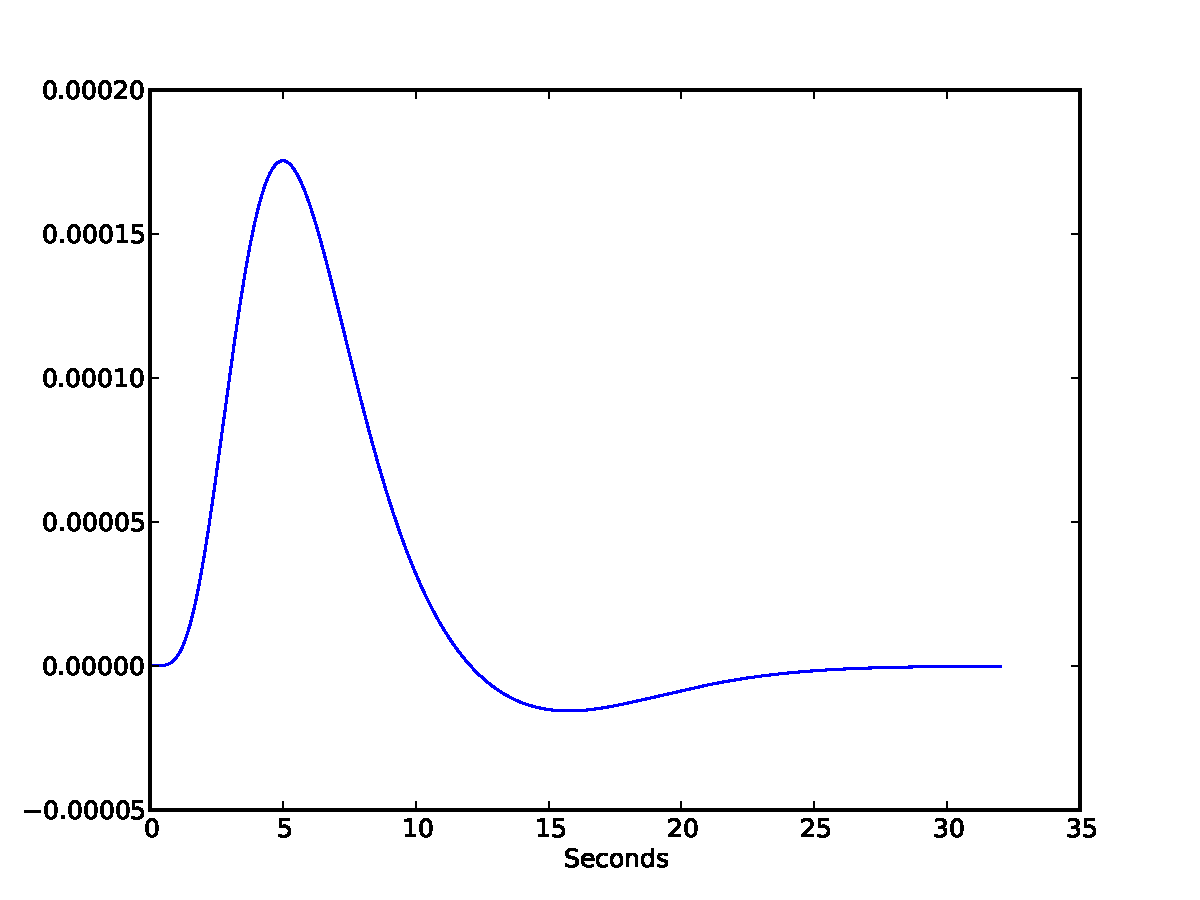
\includegraphics[scale=.7]{images/HRF}
\caption{Canonical Hemodynamic Response Function}
\label{fig:HRF}
\end{figure}

\subsection{Hierarchical Linear Models}
As mentioned previously and discussed extensively
in \cite{Friston2002} and \cite{Hofmann1997}, hierarchical models may be 
applied to account for systematic differences between subjects. For instance, if the
study happens to be a mix between young and old, incorporating
that into the model is wise, regardless if that is the purpose of the test. 
The reason to do this is to account for additional variance that may not
be present in similar studies. The Hierarchical form used by
\cite{Friston2002} is shown in \autoref{eq:Hierarchical}.

\begin{eqnarray}
\label{eq:Hierarchical}
Y(t) = X_1(t)\theta_1 + \epsilon_1(t)            \nonumber \\
\theta_1(t) = X_2(t)\theta_2 + \epsilon_2(t)     \nonumber \\
...                                              \nonumber \\
\theta_{n-1}(t) = X_n(t)\theta_n + \epsilon_n(t) 
\end{eqnarray}

The Empirical Bayes algorithm is used in both in both \cite{Friston2002} 
and \cite{Hofmann1997}. As a consequence, point estimators 
are used for each $\theta$, rather than the full distributions.

\subsection{Discussion}
\label{sec:BackgroundConclusion}
In all, the GLM is useful for determining linear 
dependence of a set of regressors on the output. Unfortunately, as discussed in
\autoref{sec:BOLD Analysis} there are significant nonlinearities 
that almost certainly cause false negatives in the Statistical Parametric
Maps. Unfortunately nonlinear analyses have only recently become feasible,
so the scale of the problem is still unknown. The problem is 
highlighted by the common scenario where no significant
activation can be found in a single run \cite{Riera2004}
\cite{Johnston2008}.  

The static nature of the  linear model also limits its inference power. 
Besides not permitting HRF differences between patients, there is no
reasonable way to incorporate other forms of physiological
data. Combined FMRI CBF or CBV imaging methods are rapidly getting better,
as seen in \cite{Chen2009}. These techniques could shed light on
neural activation by providing extra measurements, yet a 
physiologically reasonable model is necessary for this.
In reverse, activation detection methods also don't have the ability 
to identify pathologies based on state variables or parameters. For
example decreased compliance of
blood vessels could indicate, or even cause, a neurological condition that 
is not easily seen in other imaging modalities. Thus, the benefits
of physiologically meaningful models are manifold.

\section{Solving the BOLD Model}
Unlike Statistical Parametric Mapping, the techniques described in this
section are all attempts to learn some version of the BOLD model. 
Although \cite{Buxton1998} and \cite{Friston2000}
both proposed physiologically reasonable values for the model parameters, 
\cite{Friston2002b} was the first paper to calculate the parameters based 
on actual FMRI data. However, in that case, the voxels were chosen from
regions that were detected as active by the GLM. It is therefore possible
that the parameters are biased toward parameters that fit the linear model.

\subsection{Linear Approximation}
In \cite{Friston2002b}, a novel combination of linear and nonlinear modeling
was used to generate parameter estimates. Because it is impossible to 
calculate the partial derivative of
the output with respect to parameters, $\frac{\partial \theta}{\theta}$, 
\cite{Friston2002b} approximates the partial. At each step of the Expectation-
Maximization algorithm, the differential equation is integrated, calculating
the residuals. Then, for each $\theta_i$ surrounding the current estimate of 
$\theta$, a Volterra-Kernel expansion of the output $y$ is generated. Generation
of the Volterra Kernel is quick, and, since it is linear there
is an analytical solution. Thus, once the Volterra Kernel exists, the value
of $y$ at that measurement point, for that $\theta_i$ can easily be found. 
Thus, one part of the partial is calculated at one point using
$\frac{y(t) - y_i(t)}{\theta - \theta_i}$. This is repeated for
every dimension of $\theta$ to give the full $\frac{\partial y}{\theta}(t)$.
This is only at time $t$ though, and it must be repeated for every
measurement. Finally the full derivate matrix is filled out, and
the next step in the E-M algorithm can proceed. The full E-M algorithm
for estimating the states is notation-heavy and can be found in \cite{Friston2002b}.

Although this is certainly an interesting method of performing non-linear
regression, there are a few caveats. First, the partials are numerical
approximations, based on an approximate values (using Volterra-Kernels) of $y$.
Importantly, the Volterra-Expansion of $y$ is not able to model interactions
between state variables; interactions that were found to cause interesting
behavior in this work. In \autoref{sec:Unscented Kalman Filter}, for
the purpose of demonstrating nonlinearities in the signal, it was 
necessary to propagate state variables through 1 second of simulation.
For the distribution of state variables mentioned in \autoref{tab:steptable}
it was necessary to use step sizes smaller than $.001$ to prevent 
unpredictable behavior. This is using the average parameters, thus the
only complication came from the interplay between states, which can 
certainly lead to interesting behavior. Additionally, all the tests performed
in \cite{Friston2002b} were on regions found to be active by the General
Linear Model. For this reason, the reliability of the approximation is unknown
for regions that are active but
sufficiently nonlinear to avoid detection by conventional tests.

\subsection{Nonlinear Least Squares}
\label{sec:Nonlinear Least Squares}
Rather than localizing activation, by using the physiologically
plausible BOLD model, it is possible to determine the values of
governing parameters.

Although there are certainly benefits to using a derived model, rather
than a purely empirical model, there are serious implications. The
first problem is that all the powerful classical techniques of gradient
descent are off limits; since the model is a true nonlinear dynamical
system with no closed form solution. The implication of this is that
the calculation of a Jacobian for residuals won't work; and thus powerful
techniques such as the Gauss-Newton method, which are helpful in most nonlinear
problems, are off limits. Additionally, a gradient descent is difficult to
perform without the ability to form partials of the output with respect
to all the parameters. 

Although anything requiring a Jacobian is out, there are other heuristic
techniques that could potentially illuminate the BOLD response. 
Simulated Annealing (SA) is a common method of optimizing high dimensional
regression problems. The idea is to pick a random start, and then
at each iteration pick a random nearby point, and if that point is
below some energy constraint (energy is a function of the residual), 
called the temperature, the algorithm moves
to that point and continues with the next iteration. The temperature
is slowly lowered until no nearby points below the temperature can
be found (or the temperature drops below the current point). There are
variations of this, for instance it is common to require every movement
to be in the downward direction (in terms of energy). Like most nonlinear
optimization problems, there is no guarantee of an optimal solution,
although the longer the algorithm is allowed to run, the better the solution
will get. Since every step requires an entirely new run of the 
BOLD model, it can be extremely time consuming, which is why we are
not using it here.

\begin{algorithm}
\caption{Simulated Annealing Algorithm}
\label{alg:Simulated Annealing}
\begin{algorithmic}
\STATE Initialize $\Theta$, or if there exists a decent estimate start there
\STATE Initialize temperature, T to value above initial energy
\WHILE{$E(\Theta) < T$}
    \REPEAT
        \STATE Pick $\theta$ near $\Theta$
        \STATE Calculate energy, $E$, of $\theta$
    \UNTIL{$E > T$}
    \STATE Move to new estimate: set $\Theta = \theta$
\ENDWHILE
\end{algorithmic}
\end{algorithm}

%[simulated annealing image?] todo

Another potential method of interest is the use of Genetic Algorithms
(GA). Genetic algorithms are similar to Simulated Annealing, in
that they randomly move to better solutions based on a cost function.
However; in genetic algorithms a single point estimate isn't used. Instead
a population of estimates is generated, each with distinct parameters,
and then each set of parameters is rated with a fitness function. Parameter
sets that are good get a higher weight; then new parameter sets are generated by 
randomly combining pieces of the old parameter sets. The pieces are typically
chosen at a rate proportional to the fitness of the donor; thus fit
parameter sets tend to pass on their properties. In addition to this,
random mutations may be introduced that come from no existing parent. 
The new generation is then rated with the fitness function again, and
the entire process starts over. The stop condition for a genetic algorithm
is typically based on some threshold for fitness or a maximum number 
of generations. As with all nonlinear searches, unless the function is
known to be convex, there is no guarantee that a global minimum has been
reached.
%[genetic algorithm picture] todo

\begin{algorithm}
\caption{Genetic Algorithm}
\label{alg:Genetic Algorithm}
\begin{algorithmic}
\STATE Initialize $N$ estimates, $E = \{\Theta_0, \Theta_1, ... \Theta_N\}$
\FOR{G generations}
    \STATE Calculate fitness for each $\Theta$, Ex. for residual $R$, $1/R$ or, $e^{-R}$
    \FOR{$i$ in $N$}
        \STATE Randomly select two parents (with higher probability for more fit $\Theta$'s)
        \STATE Randomly merge parts of the two parents to form a new $\Theta_i$
        \STATE At some low probability change one or two parameters in $\Theta_i$
    \ENDFOR
\ENDFOR
\end{algorithmic}
\end{algorithm}

Although both these methods can be highly effective, they have the downside of
requiring very high computation time. In this case of the BOLD model,
each time the energy or fitness needs to be calculated, a large number of cycles
must be spent re-simulating the BOLD model for the set of parameters. As I'll
discuss in \autoref{sec:Particle Filter}, the Particle Filter method is able
to circumvent this re-calculation to some degree.

\subsection{Unscented Kalman Filter}
\label{sec:Unscented Kalman Filter}
The Unscented Kalman Filter (UKF) is a powerful Gaussian/Bayes filter that attempts
to model the posterior distribution of dynamical systems as a multivariate
Gaussian. The Unscented Kalman Filter (UKF) generalizes the Extended Kalman
Filter by allowing the state update to be a function, $g$,

\begin{eqnarray}
X(t) &=& g(u(t), X(t-1))\\
Y(t) &=& h(X(t)
\end{eqnarray}

In order to estimate the posterior at $t$, a deterministic set of sigma points 
(often 2 per dimension, plus 1 at the mode of the multivariate distribution)
weighted according to a Gaussian estimate of $X(t-1)$ are passed through
the update equation. This set of points are then used to estimate the 
mean and covariance of $X(t)$. The benefit of this, is that it requires
no Jacobian and only a few extra calculations to get a decent estimate of
a posterior Gaussian. In the BOLD case, the set of equations we are modeling have no 
closed form solution, and finding the Jacobian is impossible without approximations. Although 
\cite{Riera2004}, \cite{Hu2009} mention a Jacobian of the BOLD response, this is
not strictly the case and is rather $\frac{\partial J}{\partial t}$
rather than a true Jacobian.  This is important because the Extended
Kalman filter depends on the Jacobian to map a Gaussian through the 
advancement of time. Thus the popular Extended Kalman Filter won't work
in this case, whereas the Unscented Kalman Filter still does. In fact
\cite{Hu2009} uses the UKF to perform a similar type of analysis to
the one performed in this work. 

\begin{figure}
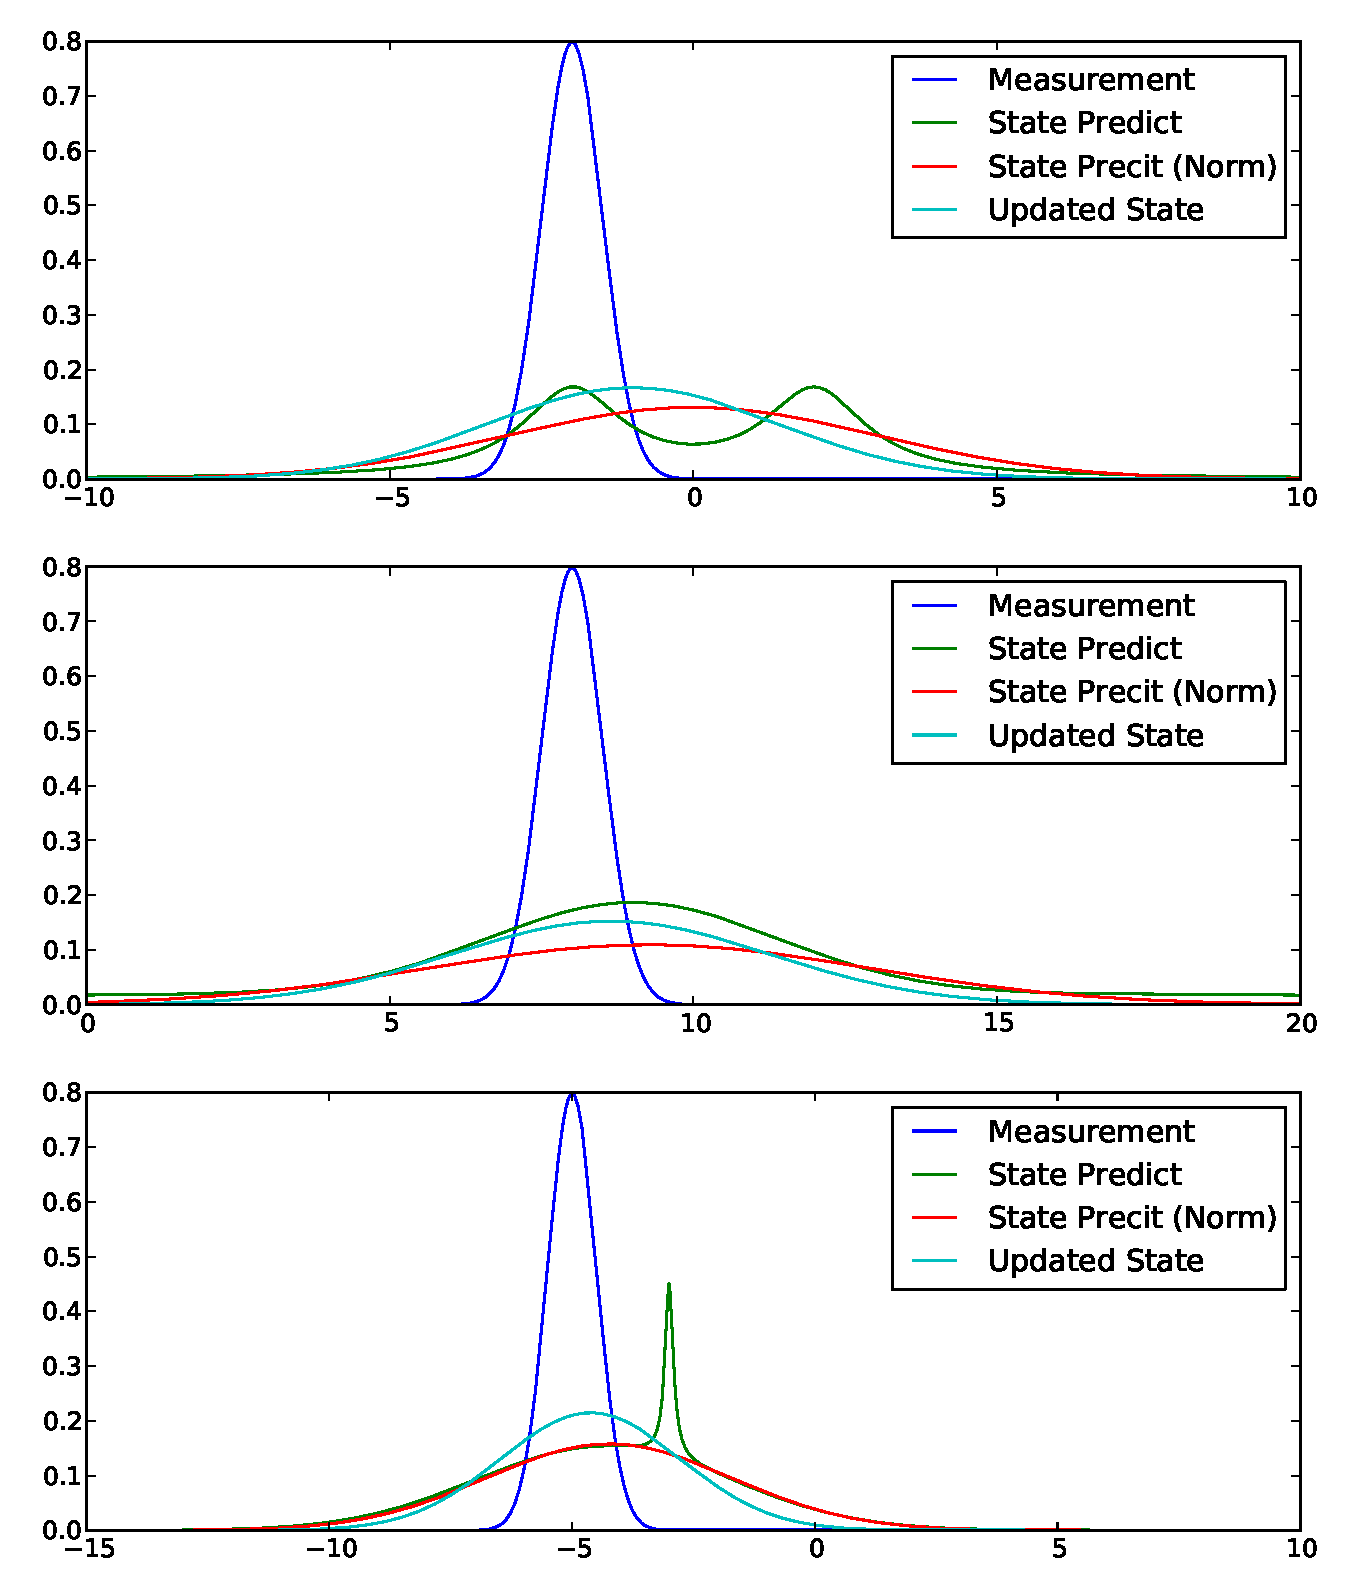
\includegraphics[width=16cm]{images/kalman}
%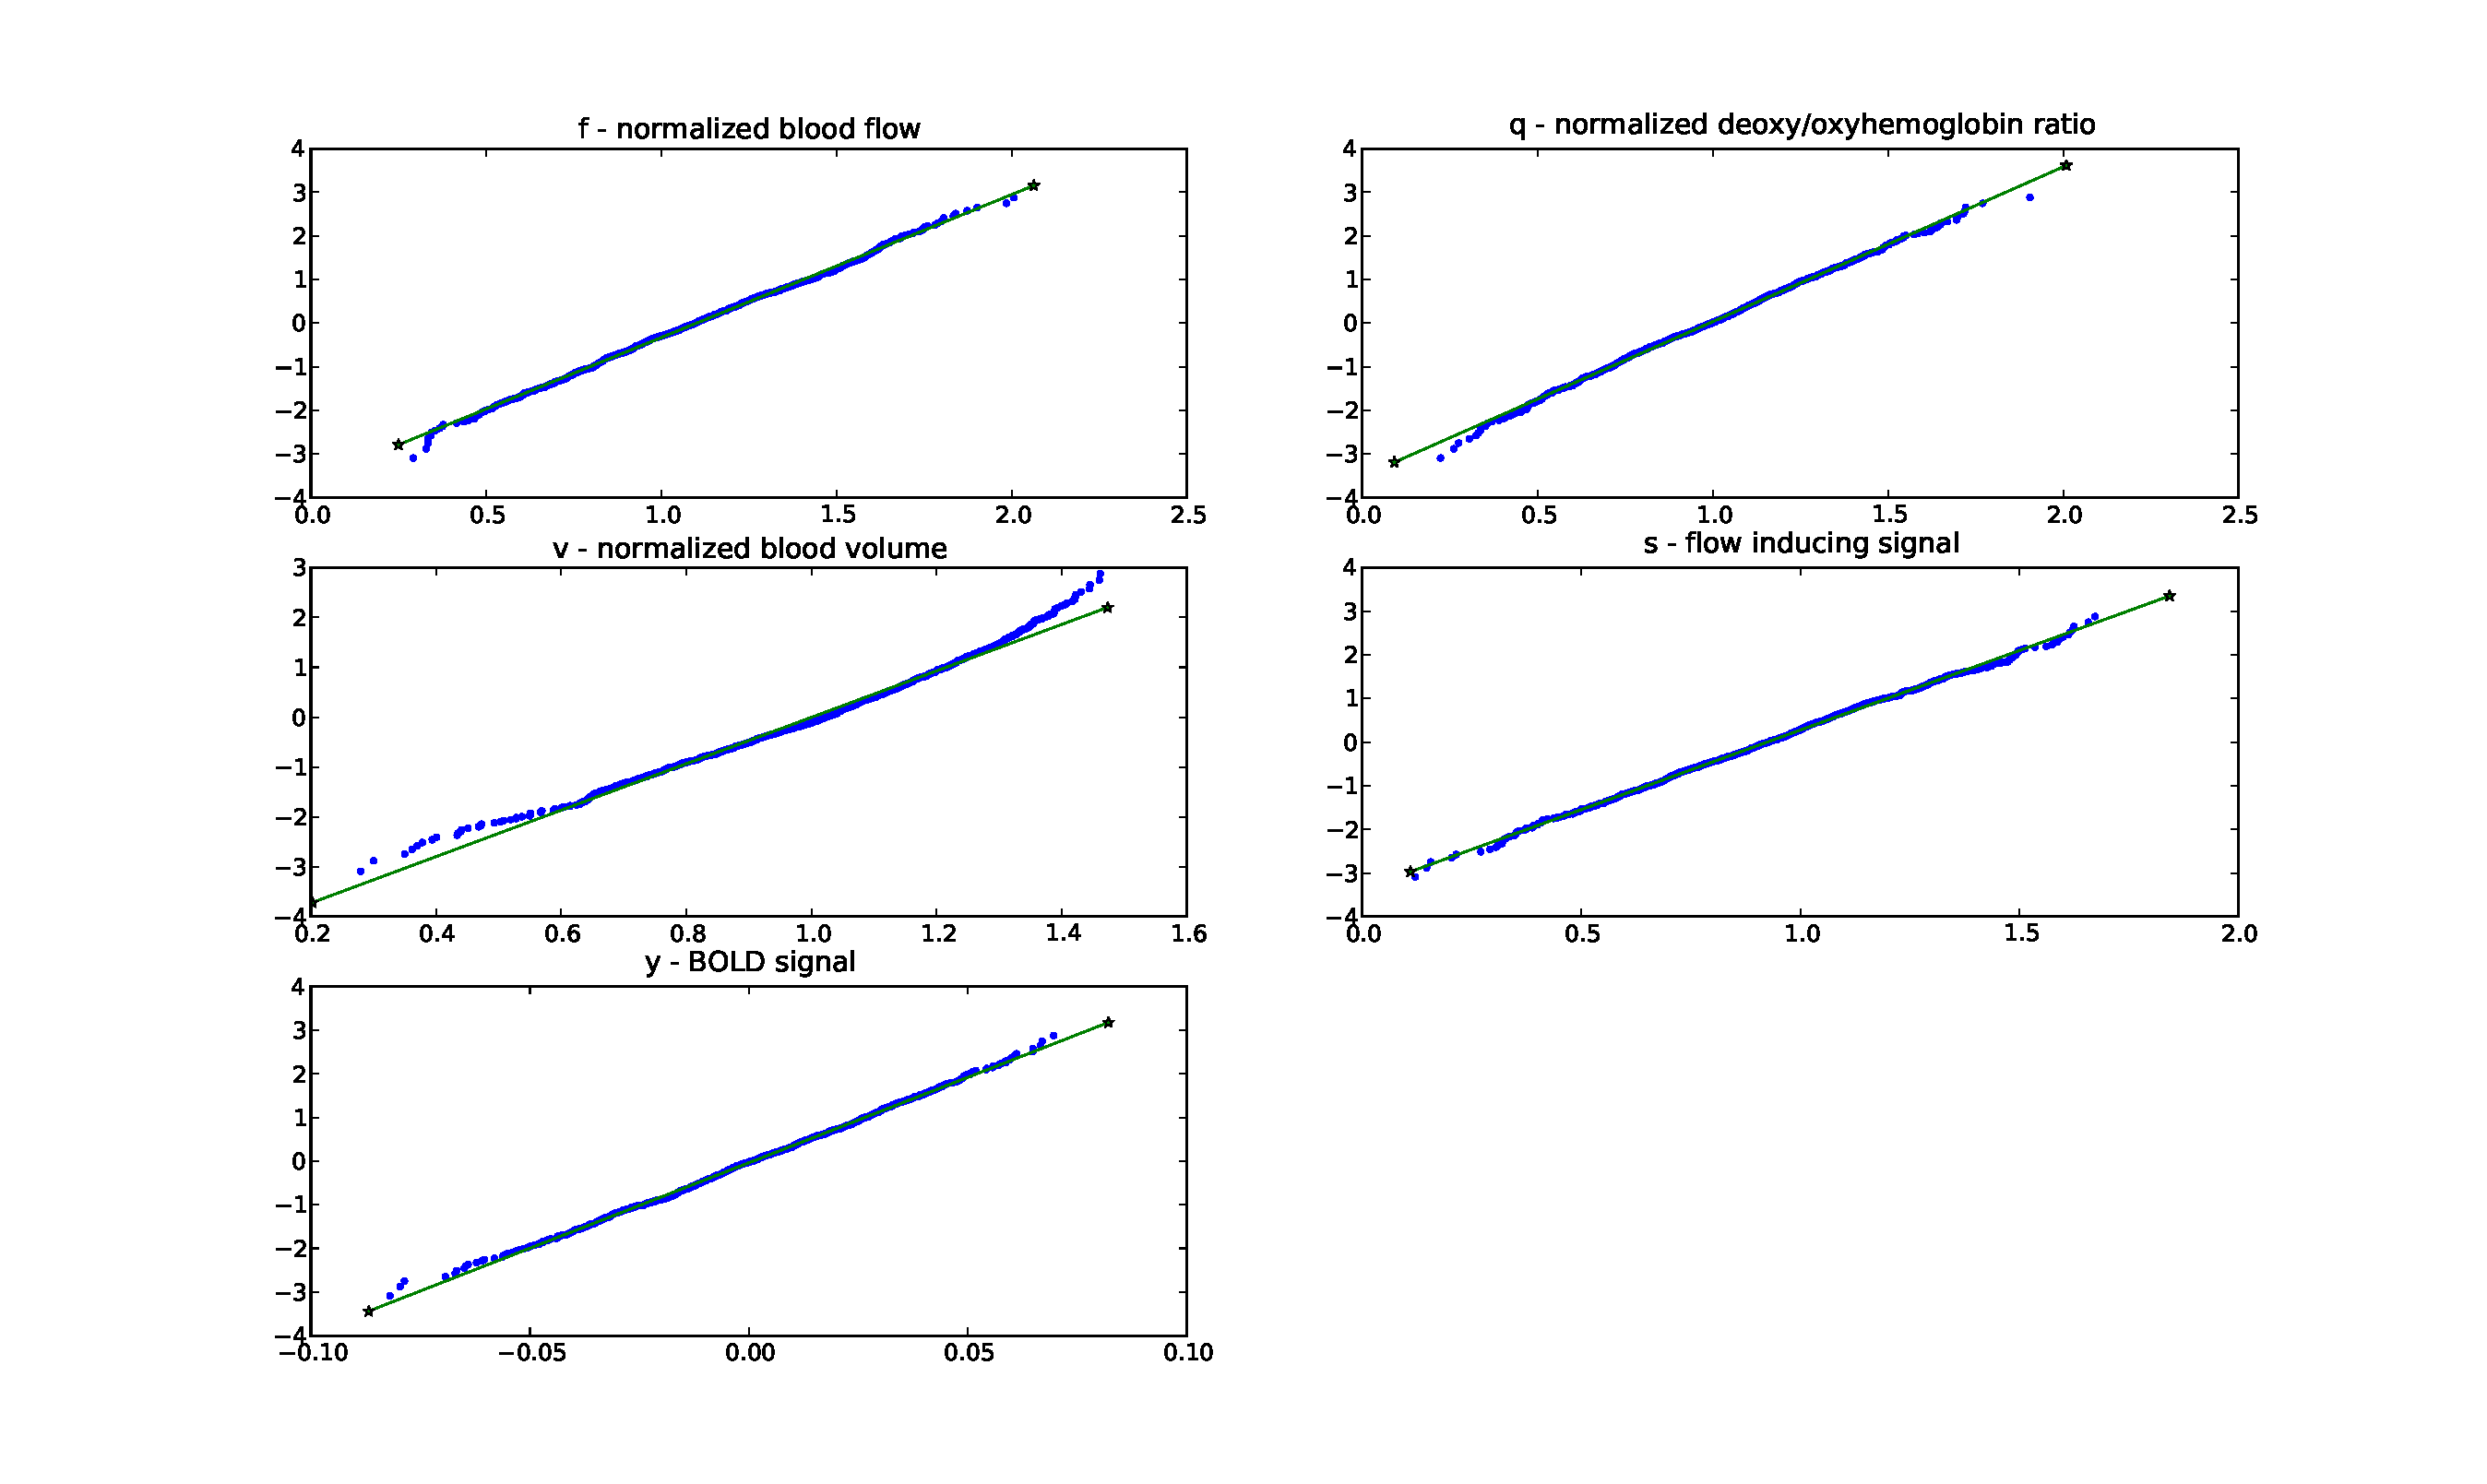
\includegraphics[trim=6cm .75cm 6cm .75cm,width=16cm]{images/gauss_step_point1sec_3sigma.pdf}
\caption{Example updates of a distribution using Kalman Filter, \cite{Thrun2005}}
\label{fig:EKFWorking}
\end{figure}

The difficulty
of using a Kalman Filter, however, is that it assumes a multivariate 
Gaussian for the state variables, $X(t-1)$. The more nonlinear the system
gets the more likely that the Gaussian will be insufficient to describe
the distribution, $X(t)$. When this occurs, every step from  $X(t+1)$ 
to $X(t)$ will introduce additional
error in the posterior distribution. Furthermore, it is not really known what 
sort of underlying distributions may exist in such a mixed biological,
mechanical, chemical system such as the brain. Assuming the parameters
all to be Gaussian may in fact be a gross error. On the other hand, for
small variances and short time steps the Gaussian distribution is a good 
fit, and so in some limited cases the Unscented Kalman Filter could work
well. These are 
non-trivial issues given that the assumption of Gaussianity is what allows
the UKF to estimate the posterior using only the first and second moments;
two parameters that don't uniquely describe most distributions.

\begin{table}[t]
\centering
\begin{tabular}{|c || c |}
\hline 
Parameter & Run 1 \\
\hline
$\tau_0$ & .98  \\
$\alpha$ & .33 \\
$E_0$ & .34  \\
$V_0$ & .03  \\
$\tau_s$ & 1.54  \\
$\tau_f$ & 2.46  \\
$\epsilon$ & .54  \\
$V_t$ & N(1, .09)  \\
$Q_t$ & N(1, .09)  \\
$S_t$ & N(1, .09) \\
$F_t$ & N(1, .09) \\
\hline
\end{tabular}
\caption{Parameters used to test Gaussianity of variables after being transitioned through
the BOLD model}
\label{tab:steptable} 
\end{table}

To determine the amount of error incurred in a Gaussian estimate during
a typical sample period, the states of BOLD equations were assigned according
to four dimensional Gaussian. The states were then propagated through two
seconds of simulation (a typical TR in FMRI) and then the resulting
marginal distributions were compared with a Gaussian distribution. The 
purpose is to determine the degree to which the results of simulation will
result in non-Gaussian output, given a Gaussian input. This also demonstrates
the degree of nonlinearity present in the system. The parameters used are 
shown in \autoref{tab:steptable}

Notably $s_t$ has intentionally been set to a non-equilibrium, but physiologically
plausible value. The value of $u$ is left at zero the entire time, so the 
system will decay naturally (see \autoref{sec:BOLD Physiology}), though initializing 
$s$ at a non-zero level will drive the system for several seconds. 
\autoref{fig:transp1s} shows the results when the system is 
left on for 100 milliseconds after setting the variables according to \autoref{tab:steptable}.
The Q-Q plots fit will with a Gaussian, demonstrating that at this short
time interval nonlinearities have not yet begun to effect the distribution.
However, \autoref{fig:trans1s} us the result after 1 second, which is faster
than most FMRI scanners are capable of sampling at. At that range the tails 
of the distributions for $v$ and $q$ are starting to deviate from the
Gaussian distribution. As a result the uncertainty in $y$ is deviating from
the Gaussian distribution as well. This is important, because although 
approximating the distribution with a Gaussian based on the first two
moments will work in the short run, there will be residual error in the
distribution. 

On the other hand, this effect is more limited if the initial variance is somewhat
smaller. In tests with those cases, it took much longer for the nonlinearities to skew
the distribution. That result could be encouraging to those looking to use the
UKF, if the distributions are kept relatively thin.

Another potential problem with the UKF is that typically the sigma points,
used to estimate the posterior probability, $P(X(t) | X(t-1), u(t))$, are
located on the main axes. As a result, the covariances are not allowed to 
be effected by the state transition the same way the variances are. While
this may be reasonable in low-dimensional systems, high dimensional systems
have a much greater potential for interplay between the variables. While
this problem is simple to fix (by using more sigma points off
the main axes), there is a definite cost in complexity.

Ultimately, there is a distinct possibility that the nonlinearities of 
the BOLD model make Gaussian estimates unrealistic and thus less effective.
More advanced tests where static variables such as $\alpha$ are varied
as well could shed even more light on the issue. The trouble with using
the UKF then to estimate parameters is that all eleven members of $X$ would
be treated like a single joint Gaussian distribution which certainly 
compound the issues of nonlinearity seen in \autoref{fig:transp1s} and 
\autoref{fig:trans1s}

\begin{figure}
\centering
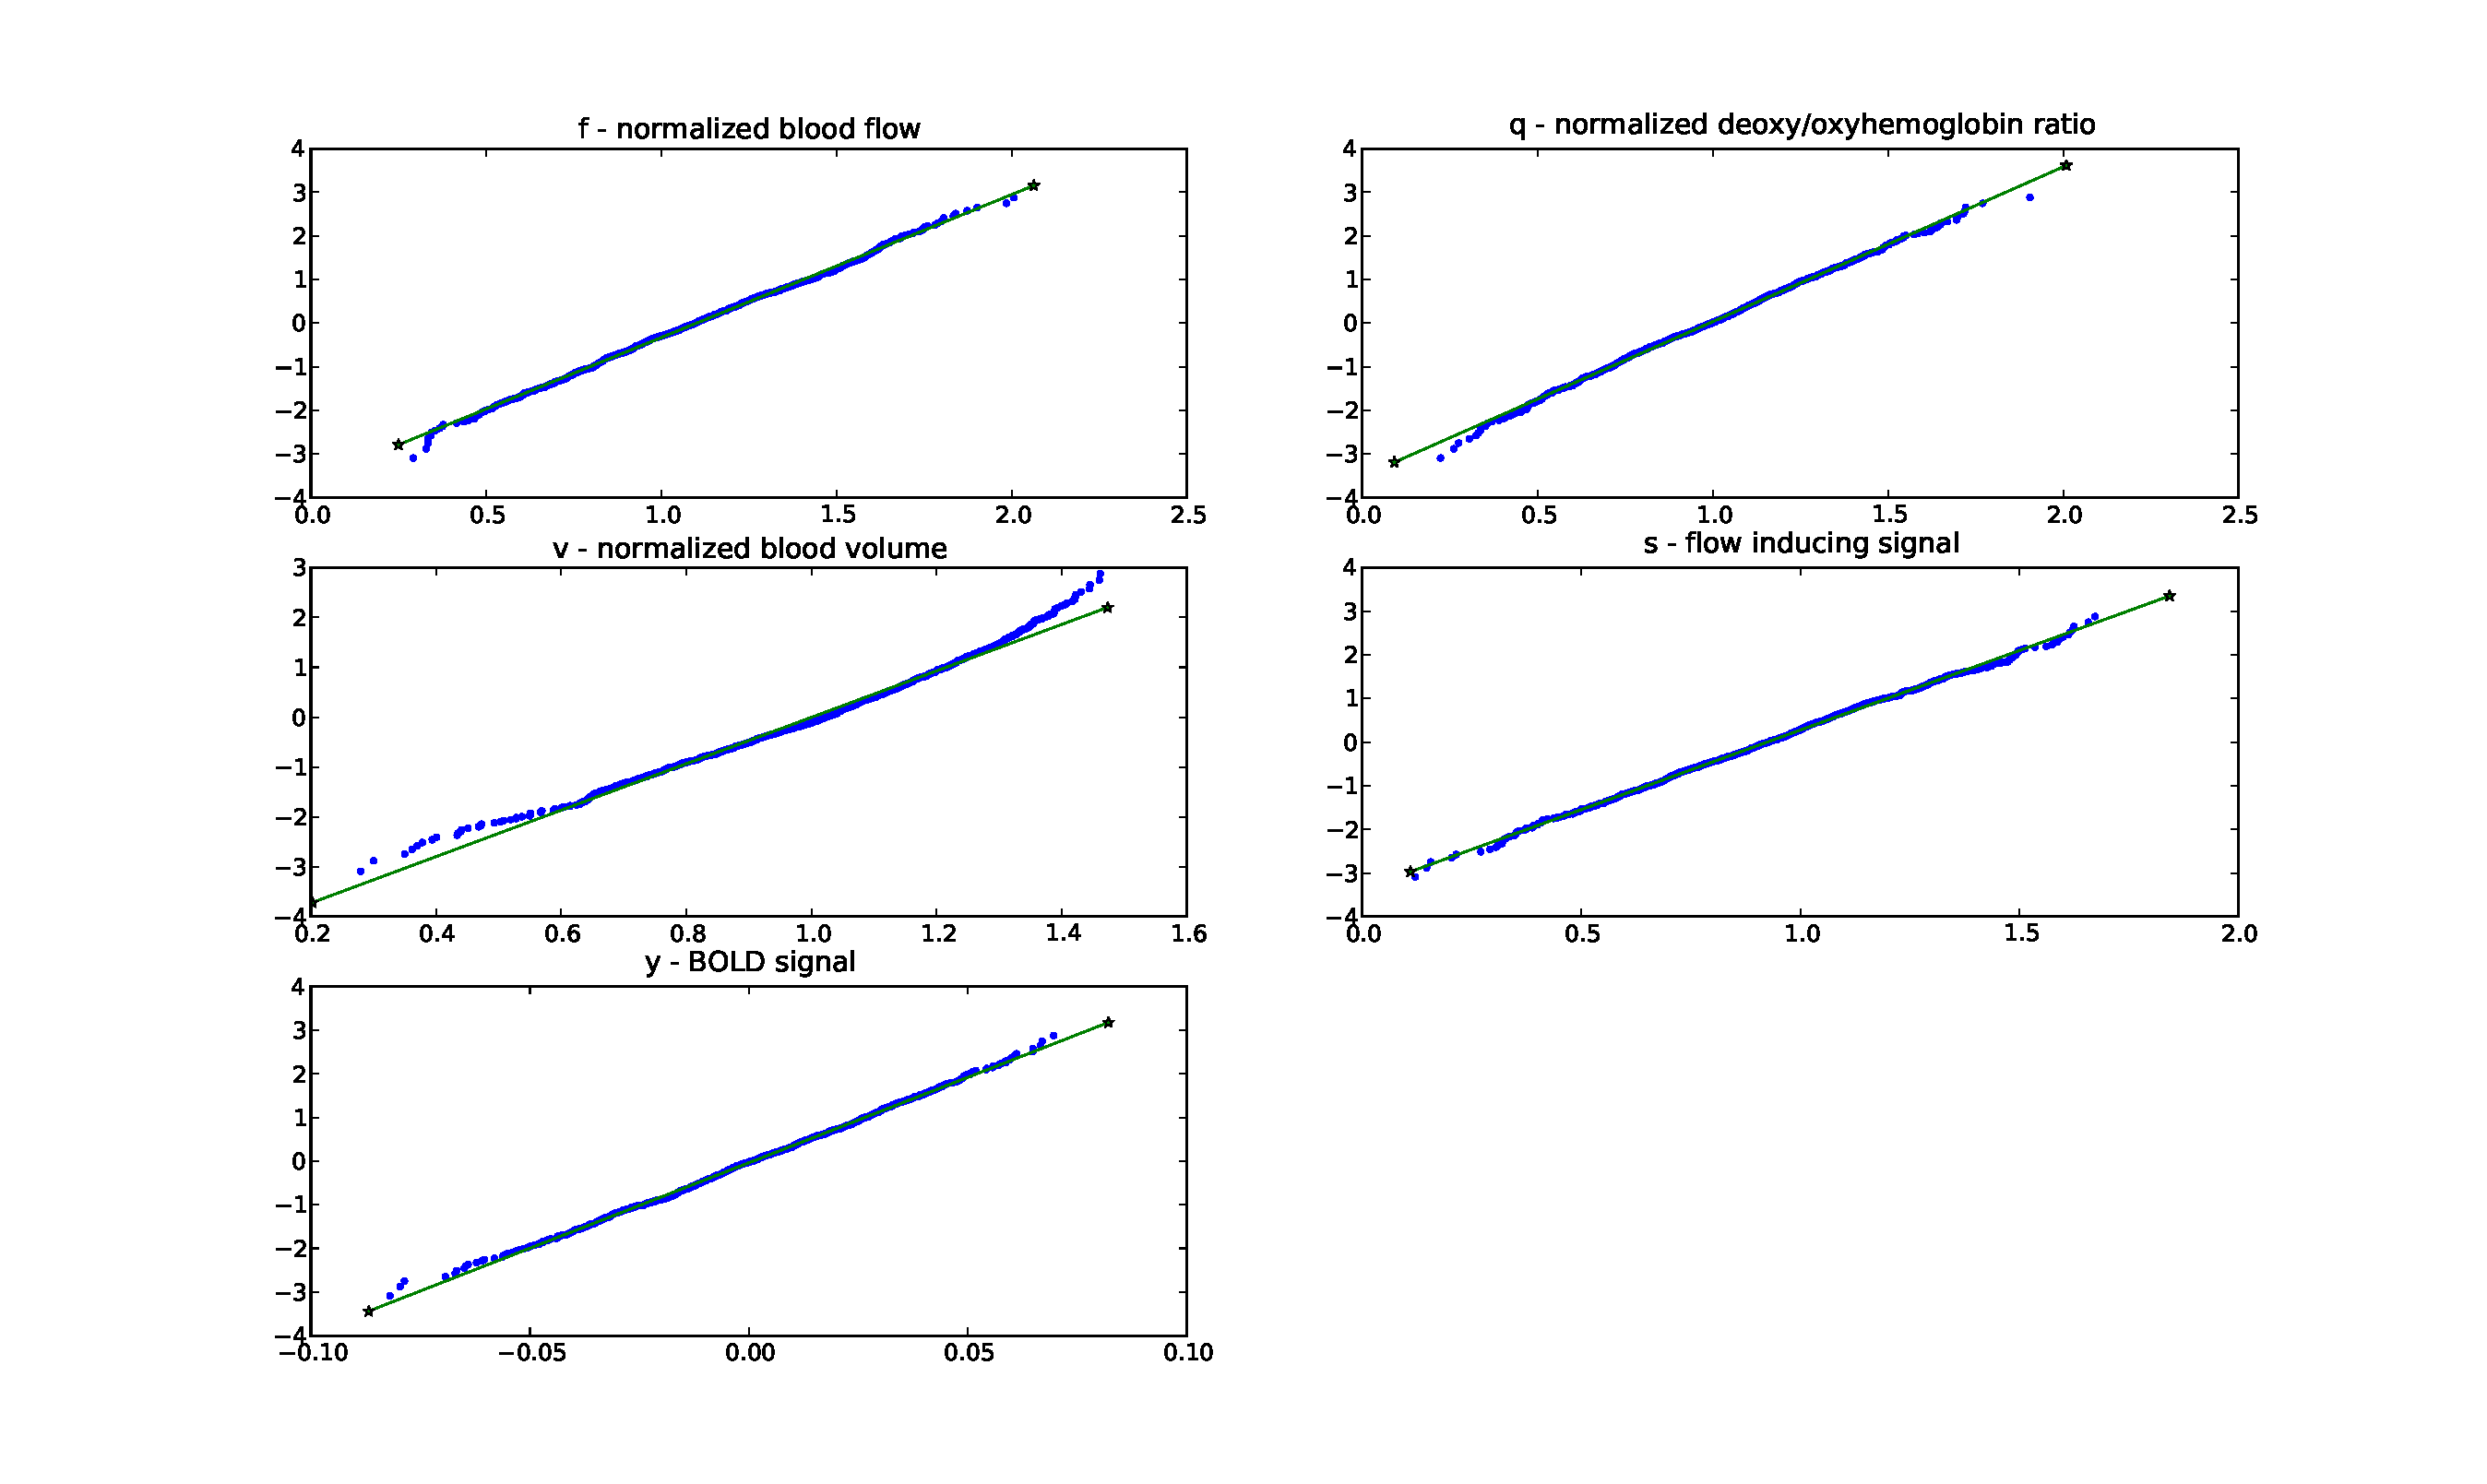
\includegraphics[trim=6cm .75cm 6cm .75cm,width=16cm]{images/gauss_step_point1sec_3sigma.pdf}
\caption{Distributions of state variables after simulating for .1s}
\label{fig:transp1s}
\end{figure}

\begin{figure}
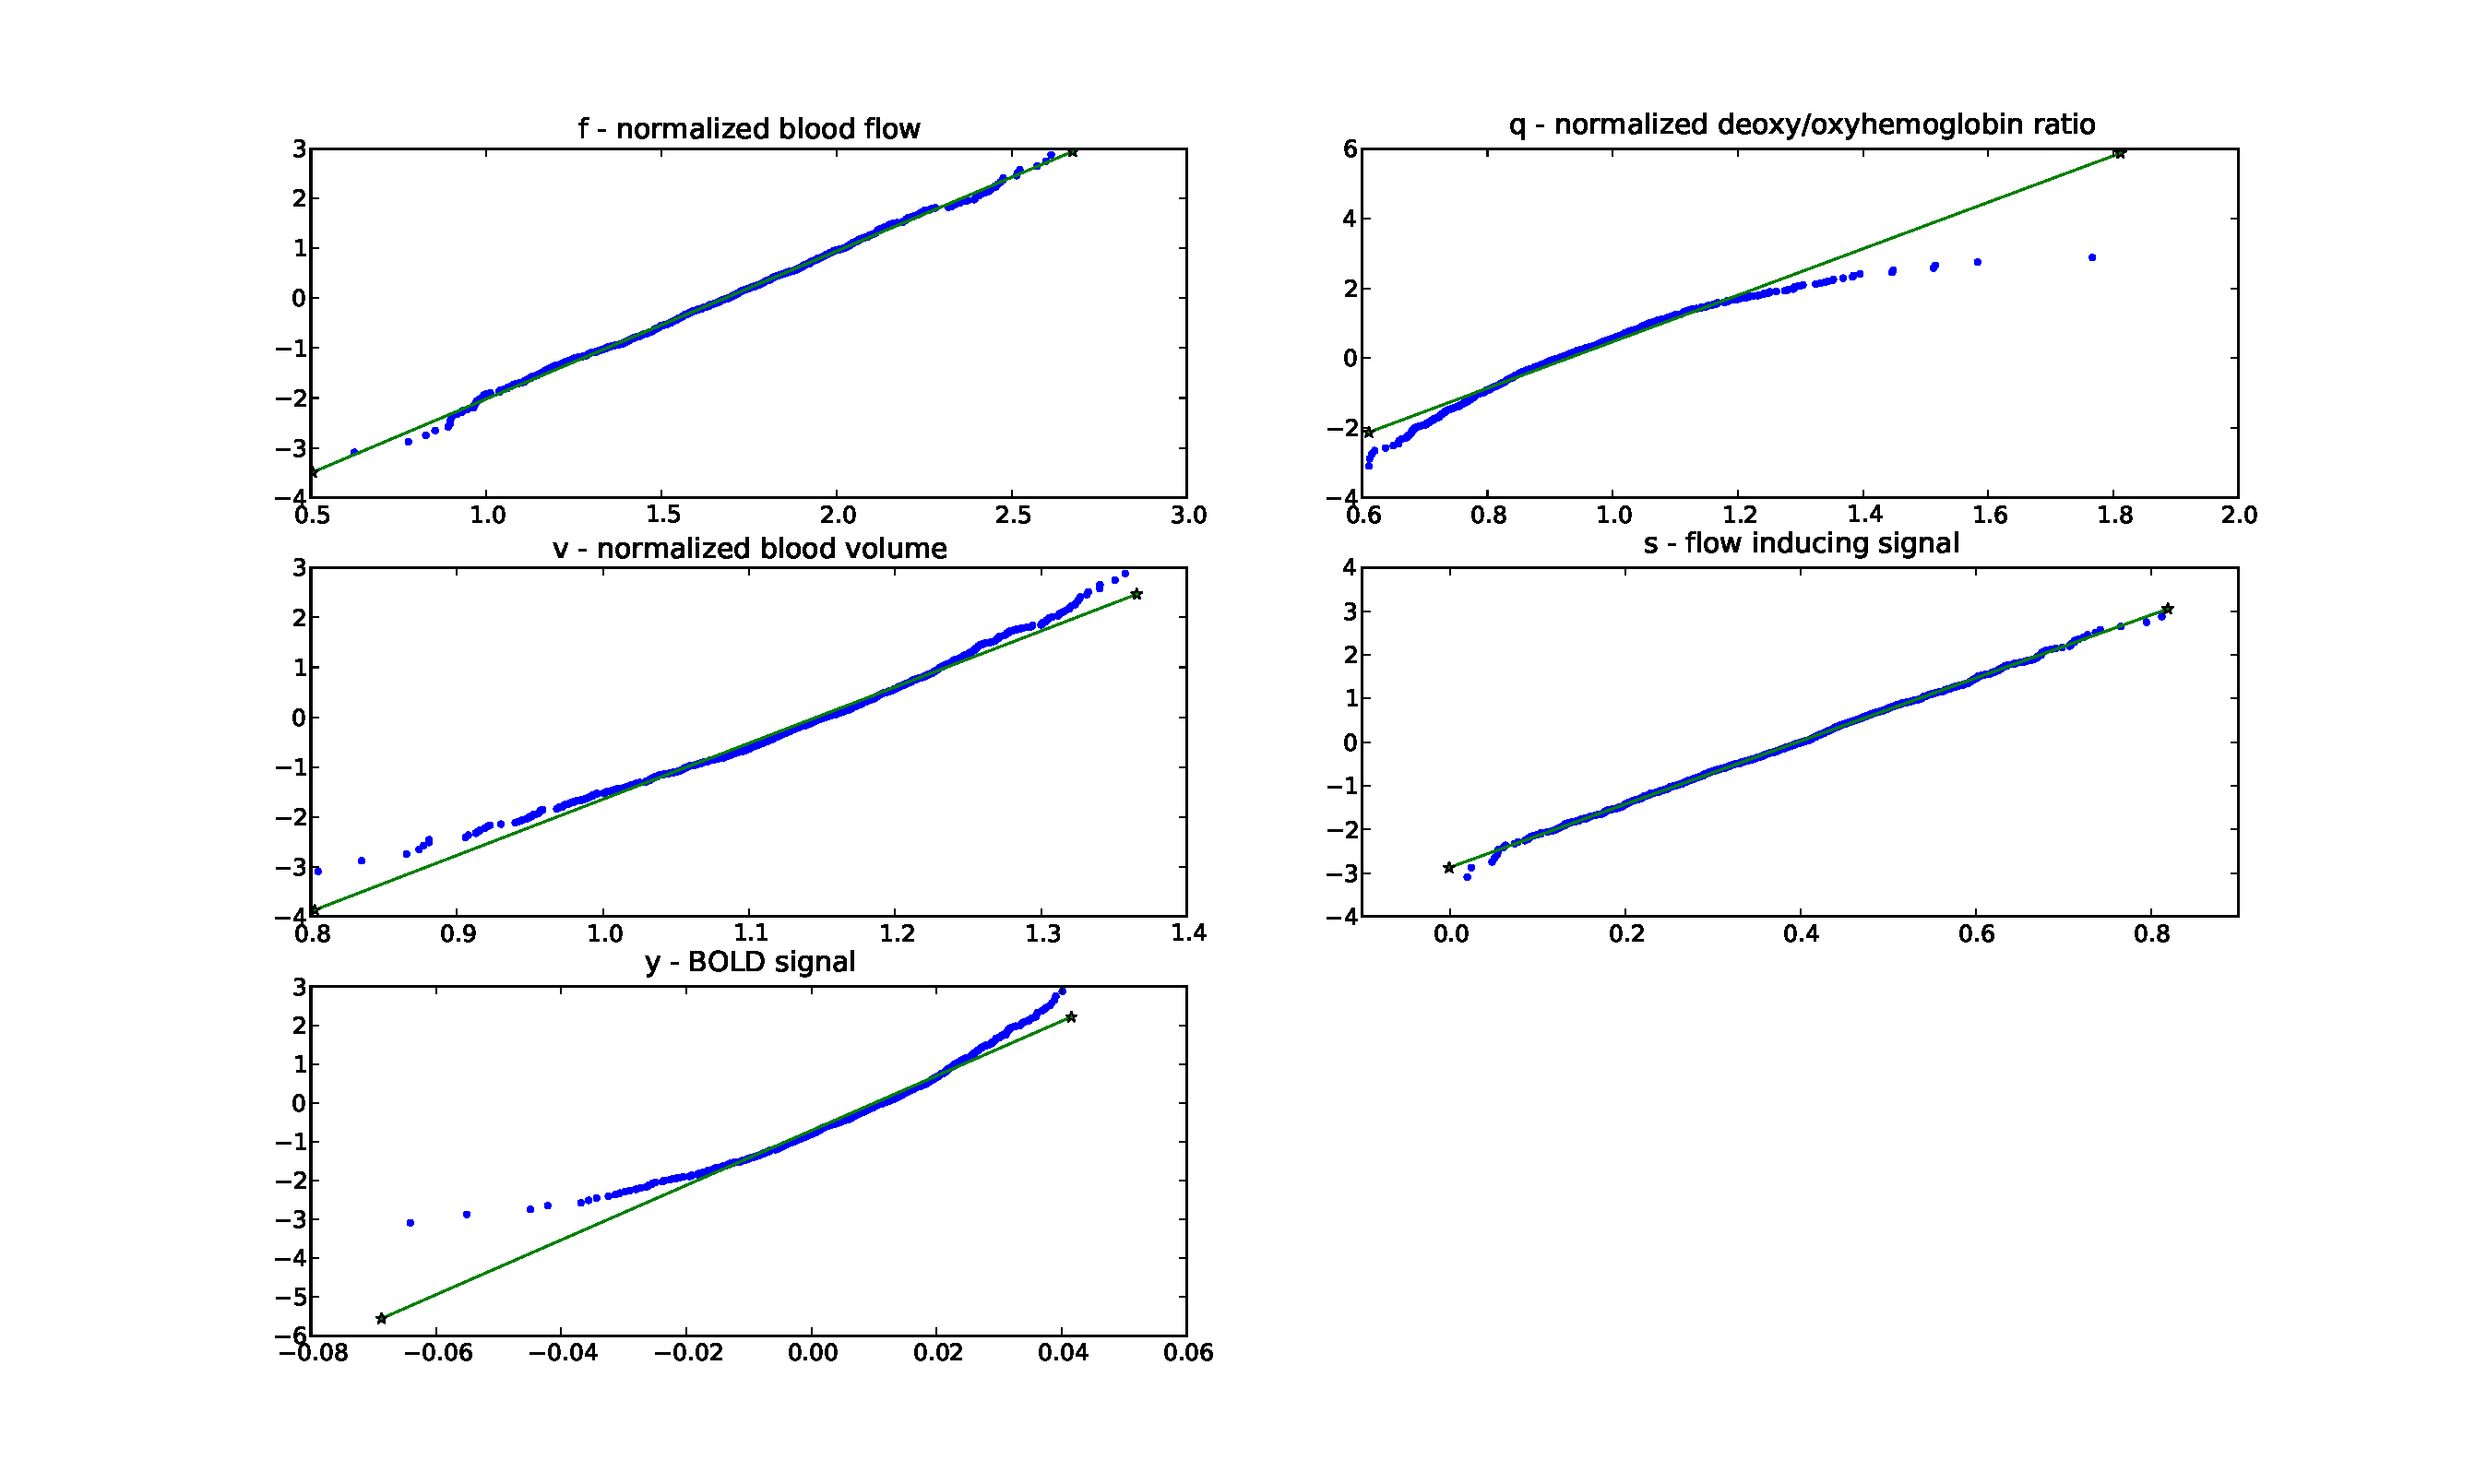
\includegraphics[trim=6cm .75cm 6cm .75cm,width=16cm]{images/gauss_step_1sec_3sigma.pdf}
\caption{Distributions of state variables after simulating for 1s}
\label{fig:trans1s}
\end{figure}

\subsection{Hybrid Methods}
In \cite{Riera2004}, a maximum
likelihood method for innovation processes was used, as described by
\cite{Ozaki1994}. \cite{Ozaki1994} uses a similar construction to a 
Kalman filter, to break the time series into a series of innovations,
for which Maximum Likelihood was performed. While this is probably the most
likely solution to give the correct output, there are a few problems. First, every
step in parameter space requires a recalculation of all the state variables. With
two or three parameters this is fine, more than that, and calculations can become
intractable. Additionally, there is no way to ensure a global minimum is reached.
Although this is also true of the methods in \autoref{sec:Nonlinear Least Squares},
those methods contained random elements designed to overcome this issue.

In \cite{Johnston2008}, a hybrid particle filter/gradient
descent algorithm was used to simultaneously derive the static and dynamic 
parameters, (classically known as parameters and state variables, respectively).
A particle filter is used to calculate the state variables at each
time; then the estimated distribution of the particles is used to find
the most likely set of parameters that would give that distribution of state variables.
This process is repeated until the parameters converge. Interestingly
\cite{Johnston2008} comes to a very different set of parameter estimates as compared
to the original \cite{Friston2000} estimates (\autoref{tab:Params}). In fact the results 
are significantly different from virtually every other study. The most obvious discrepancy
is the larger time constants, $\tau_f$, $\tau_s$ and $\tau_0$. 
While of course this could be poor convergence of the algorithm, there is another other possibility.
Unlike all the other methods mentioned, excepting the methods in \autoref{sec:Nonlinear Least Squares},
the algorithm described in \cite{Johnston2008} does not depend on prior distributions.
It is possible then that the bias toward the prior in other methods screwed the results. 
While \cite{Johnston2008} is certainly in the minority; further exhaustive studies 
of the parameters, using unbiased techniques may be called for. A further 
comparison between the distributions found in \cite{Johnston2008} and 
\cite{Friston2000} will be discussed in \autoref{sec:PriorDist}, including
graphs: \autoref{fig:MeanResponseF}, \autoref{fig:MeanResponseJ}.

\section{Conclusion}
There is no ideal solution to solving this system of nonlinear
equations. Exhaustive search type methods such as those employed by
\cite{Johnston2008} and \cite{Vakorin2007} have long
run times even for a single voxel. While Volterra models are an interesting
solution,there have not yet been exhaustive tests to determine whether
such approximations work well throughout state space. The most promising
method of those reviewed here is the Kalman filter based method. It is
able to maintain a fast runtime while still approaching the solution.
While the reliance on a Gaussian estimate to the true posterior distribution could
cause problems, some modifications could make it powerful. 
The particle filter method proposed in the next section bears a strong 
resemblance to the unscented Kalman filter; albeit with more point estimating
the posterior. 
